\documentclass[10pt,oneside,a4paper, twocolumn]{article}
\usepackage{graphicx}

\usepackage{hyperref}
\usepackage{subcaption}
\usepackage{caption}
\usepackage{cuted}

\title{Integrating Knowledge Graphs into the Debian Ecosystem}
\author{Alexander Belikov \\ \href{mailto:alexander@growgraph.dev}{alexander@growgraph.dev}}
\date{June 2025}

\begin{document}

    \maketitle

    \begin{abstract}
        In an era where software systems are increasingly complex and interconnected, effectively managing the relationships between packages, maintainers, dependencies, and vulnerabilities is both a challenge and a necessity.
        This paper explores the integration of knowledge graphs into the Debian ecosystem as a powerful means to bring structure, semantics, and coherence to diverse sources of package-related data.
        By unifying information such as package metadata, security advisories, and reproducibility reports into a single graph-based representation, we enable richer visibility into the ecosystem's structure and behavior.
        Beyond constructing the Deb-KG graph, we demonstrate how it supports practical, high-impact applications — such as tracing vulnerability propagation and identifying gaps between community needs and development activity — thereby offering a foundation for smarter, data-informed decision-making within Debian.
    \end{abstract}


    \section{Introduction}
    Knowledge graphs (KGs) are structured representations of entities and their interrelations, rooted in semantic web principles.
    They have gained significant traction across domains — from powering search engines and virtual assistants to supporting knowledge management in fields such as agriculture~\cite{Min2022-ff} and software engineering~\cite{Chen2023-pe}, as well as in academic domain with an application resource allocation\cite{xsi}.
    By integrating diverse data sources into a unified semantic model, KGs enable complex queries, inference, and decision support.

    Software ecosystems, in particular, stand to benefit from this approach.
    These ecosystems encompass intricate interdependencies between packages, maintainers, vulnerabilities, licenses, and community contributions.
    A knowledge graph provides a powerful abstraction to capture and analyze these relationships, enabling improved governance, automation, and resilience.

    The Debian operating system, a foundational distribution in the free software world, exemplifies such complexity.
    With over 50,000 packages maintained by a distributed network of contributors, Debian embodies a richly interconnected environment.
    Dependencies among packages, propagation of security fixes, reproducible builds, and human collaboration patterns all contribute to a system that is both large-scale and socially maintained.

    We introduce \emph{Deb-KG}, a knowledge graph constructed for the Debian ecosystem using the GraphCast ingestion framework~\cite{graphcast}.
    Deb-KG integrates package metadata, security advisories, reproducibility reports, and community signals into a coherent property-graph model.
    This enables a range of applications, including:

    \begin{itemize}
        \item Tracing downstream packages affected by vulnerabilities to support timely patching;
        \item Auditing license compatibility across dependency chains;
        \item Profiling maintainer expertise to inform mentorship and delegation;
        \item Monitoring reproducibility status across package clusters;
        \item Connecting external inputs (e.g., feature requests or community proposals) to inform prioritization and engagement strategies.
    \end{itemize}

    These applications highlight the need to optimize Debian workflows not only for efficiency but also for robustness, prioritization, and proactive planning.
    A KG approach enables the system to learn from external signals — such as unreported bugs or unmet user needs — and to surface critical implicit interactions between code and contributors, particularly those involving domain-specific expertise.

    Throughout this paper, we define a knowledge graph as a set of typed vertices and edges, where both entities and relationships carry properties.
    Our use of the property graph model reflects a preference for tractable computation and integration over exhaustive ontological description, aligning with the practical demands of large-scale software ecosystems.


    \section{Deb-KG Schema}

    The Debian ecosystem is centered around packages and the complex web of relationships between them.
    Beyond the standard \texttt{Depends} relation, Debian supports several other dependency types, including \texttt{Recommends}, \texttt{Suggests}, and \texttt{Pre-Depends}, each conveying different semantic strength in package coupling.

    Packages are developed, maintained, and updated by maintainers — who may be individuals or teams.
    Users interact with packages primarily through installation and usage, often reporting bugs that are associated with specific versioned packages.
    These bug reports may lead to fixes, feature changes, and ultimately the release of new package versions, see Fig.\ref{fig:schema}.

    In addition to these explicit relationships, there are numerous implicit ones.
    For example, packages may fulfill similar functional roles (e.g., multiple image viewers), exhibit similar usage patterns, or be maintained by contributors with overlapping areas of expertise.
    Capturing these latent dimensions is essential for understanding workflow dynamics and community structure.

    To model this schema and transform raw data into a graph database, we use GraphCast~\cite{graphcast} — a declarative framework for ingesting tabular and hierarchical data sources (e.g., JSON, XML) into property graphs.

    Our data sources include:
    \begin{itemize}
        \item A Debian package mirror (\url{http://deb.debian.org/debian}) for package metadata and maintainer information;
        \item The Debian Bugs SOAP API (\url{https://bugs.debian.org/cgi-bin/soap.cgi}) for structured bug report data.
    \end{itemize}

    The dependency structure among packages forms a directed acyclic graph (DAG), reflecting build and installation order constraints.
    Maintainer relationships introduce additional complexity, as a package may be co-maintained or transferred between individuals and teams over time.

    This schema serves as the foundation for Deb-KG, enabling rich semantic representation of technical and social structures within Debian.
    The code for data collection and knowledge graph construction is provided in a github repository: \url{https://github.com/alexander-belikov/deb-kg}.


    \begin{strip}
        \centering
        \begin{subfigure}[t]{0.75\textwidth}
            \centering
            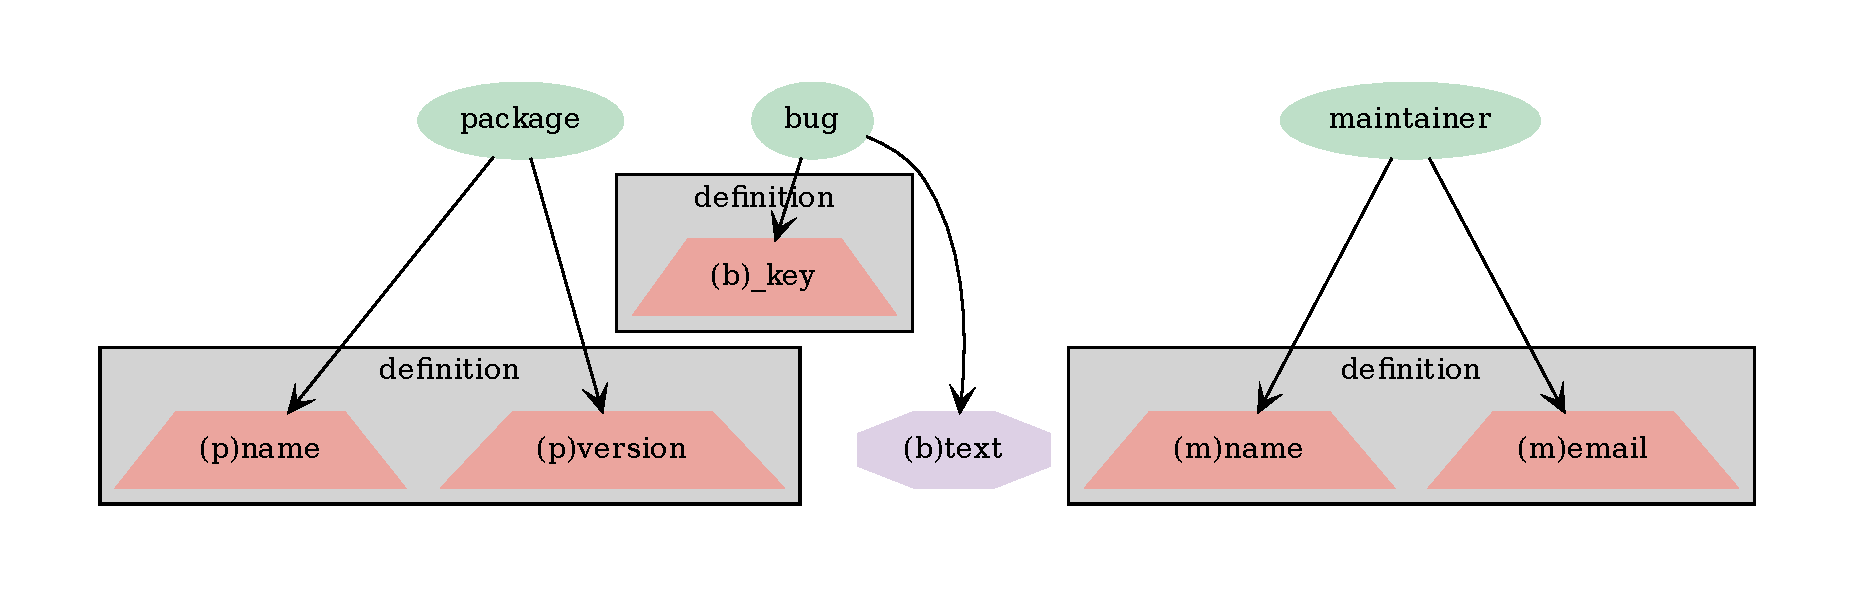
\includegraphics[width=\textwidth]{../figs/debian-eco-vc2fields}
        \end{subfigure}%
        \hfill
        \begin{subfigure}[t]{0.23\textwidth}
            \centering
            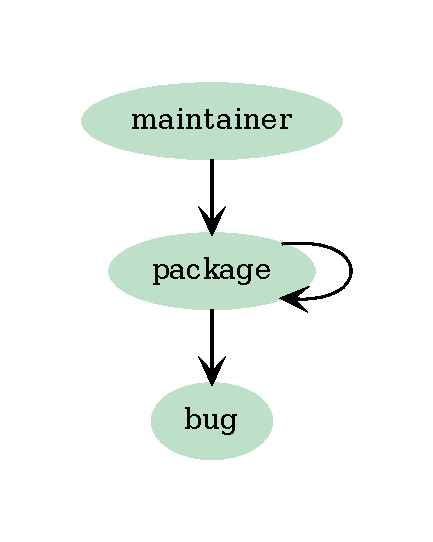
\includegraphics[width=\textwidth]{../figs/debian-eco-vc2vc}
        \end{subfigure}

        \captionof{figure}{Schema components in Deb-KG. \textbf{Left:} Internal structure of entities: \texttt{Package}, \texttt{Maintainer}, and \texttt{Bug}. \textbf{Right:} Relations between packages.}
        \label{fig:schema}
    \end{strip}

    \section{Practical Applications}


    {\bf Vulnerability Propagation and Prioritization}: Deb-KG enables tracing how security vulnerabilities propagate through the Debian ecosystem by modeling packages and their dependencies as a directed graph. Each package is linked to its known bugs (including CVEs) and to other packages via versioned dependency edges. In this structure, a vulnerability in a core package — such as a C library or compression tool — can be traced forward to identify all transitive downstream packages that rely on it, either directly or indirectly.

    This facilitates rapid assessment of impact and helps prioritize which vulnerabilities demand immediate attention. For example, if a vulnerability affects \texttt{libssl}, the graph can enumerate all packages that eventually depend on it, highlighting critical infrastructure components (e.g., web servers, network tools, or authentication libraries). This waterfall effect, often difficult to quantify manually, becomes immediately visible in Deb-KG’s queryable structure.

    Furthermore, by integrating package popularity metrics (e.g., installation counts) and metadata such as last update date or maintainer availability, one can rank affected packages based on real-world usage and maintenance capacity. This supports risk-aware patch scheduling and coordination between maintainers of interdependent packages.

        {\bf Mapping Community Needs and Engagement Gaps}: Deb-KG also supports the mapping of unmet community needs by linking Debian packages to external platforms where users and developers express requests, ideas, or feedback. For instance, proposals from the “grow-your-ideas” platform or feature discussions from mailing lists can be semantically aligned to packages in the knowledge graph.

    Once these links are established, one can identify packages that have accumulated significant user interest but show little recent development activity, few maintainers, or a backlog of unresolved bugs. This provides a data-driven view into attention gaps within the ecosystem.

    Moreover, the graph can highlight mismatches between user demand and maintainer coverage — e.g., a high-priority package used in scientific computing that lacks active stewardship.
    This insight can inform outreach efforts, mentorship programs, or targeted funding, and even guide where to route new contributors based on their interests and background.

    By embedding both technical and social signals, Deb-KG acts as a socio-technical observatory, helping the community align development resources with real-world usage and demand.


    \section{Conclusion}

    We presented Deb-KG, a property graph constructed from Debian’s package ecosystem.
    It captures key entities and relationships — including packages, maintainers, bugs, and dependencies — and serves as a foundation for both optimization workflows and the development of more detailed semantic schemas.

    Future improvements involve work along two main directions: enhancing the representation of the ecosystem, and building decision-support tools for resource allocation.

    \begin{itemize}
        \item \textbf{Temporal modeling}: Software development is inherently temporal.By incorporating timestamps for bug reports, package uploads, and version changes, we can model event sequences and enable time-aware analysis and predictive modeling.

        \item \textbf{Integration of external data}: Incorporating additional data sources — such as security advisories from upstream projects, user feedback platforms, or academic impact metrics — can enrich the graph and expose otherwise hidden signals.

        \item \textbf{Semantic similarity of packages}: Using static analysis or metadata inspection, we can infer functional similarity between packages (e.g., alternative web browsers or image viewers), aiding in tasks like replacement suggestions or diversity audits.

        \item \textbf{Fine-grained code structure}: Future versions may introduce nodes for internal entities such as software functions or code patterns, allowing deeper program analysis and technical debt tracking.

        \item \textbf{License normalization}: Unifying license data into canonical types can facilitate accurate transitive license auditing and conflict detection across dependency trees.
    \end{itemize}

    As the graph evolves, it will incorporate more cycles, richer edge types, and semantically inferred links — gradually transitioning from a dependency DAG to a fully interconnected socio-technical knowledge graph.

    In parallel, we aim to develop resource allocation models that leverage this graph structure.
    Such models can guide decisions on bug triaging, package upgrading or deprecation, maintainer support, and coordination across subsystems.
    For example, one could compute an optimal portfolio of bugs to resolve given constraints on developer time, or identify high-impact packages requiring intervention due to both technical fragility and social under-maintenance.

    Finally, tools like Deb-KG can support multi-objective optimization — not only in terms of time and robustness, but also incorporating ethical dimensions such as equitable contribution, open licensing, and environmental or academic impact.
    Knowledge graphs provide the expressive substrate needed to reason about such multi-dimensional trade-offs at scale.


    \bibliographystyle{unsrt}
    \bibliography{refs}

\end{document}
